\documentclass[12pt,twosides,onecolumn,openany]{article}
\usepackage{graphicx} 
\usepackage[catalan]{babel}
\usepackage{emptypage}
\usepackage{hyperref}
\usepackage{mathtools}
\usepackage{blindtext}
\usepackage[utf8]{inputenc}
\usepackage{caption}
\usepackage{subcaption}
\usepackage{wrapfig}
\usepackage[a4paper]{geometry}
\geometry{top=2.5cm, bottom=2.5cm, left=2.5cm, right=2.5cm}
\usepackage{fancyhdr}
\pagestyle{fancy}
\usepackage{amsmath}
\usepackage{amssymb}
\usepackage{amsfonts}
\providecommand{\norm}[1]{\lVert#1\rVert}
\hypersetup{colorlinks=true,urlcolor=blue,linkcolor=blue}
\usepackage{multirow}
\usepackage{multicol}
\usepackage{rotating}
\usepackage{titlesec}

\newenvironment{Figura}
  {\par\medskip\noindent\minipage{\linewidth}}
  {\endminipage\par\medskip}

\titleformat{\section}  % comando de sección a formatear
  {\fontsize{14}{16}\bfseries} % formato para toda la línea
  {\thesection} % cómo mostrar el número
  {0.4em} % espacio entre el número y el texto
  {} % formato solo para el texto
  [] % formato para después del texto


\fancyhf{}
\fancyhead[RO,LE]{Lliurament 2}
\fancyhead[LO,RE]{Termodinàmica i Mecànica Estadística}
\fancyfoot[RO,LE]{\thepage}
\graphicspath{ {images/} }

\begin{document}

\begin{center}
    {\Large \textbf{Termodinàmica i Mecànica Estadística}}\\
    \vspace{0.2cm}
    {\large Segon Lliurament}\\
    \vspace{0.2cm}
    Autor: Miguel A. (1637738)\\
    {\footnotesize Data: 22.12.24}
\end{center}
\textit{Model unidimensional de macromolècula. col·lectivitat Canònica.} Considereu el polímer unidimensional anterior. L'apliquem una força externa $f$ als seus ectrems (per exemple, l'hi pengem un pes), de forma que l'energia del polímer serà $E=-fR$. Trobeu:\\\\
\textbf{a) La funció de partició de la cadena.}\\\\
Al treballar amb una macromolècula amb un nombre enter de segments i el seu comportament treballem amb un sistema discret. Aplicar una força externa ens permet treballar amb la col·lectivitat canònica. Notem com, aquest context de sistema discret correspon al context de Maxwell-Boltzmann, per tant, podem calcular la funció de partició del sistema a partir de la funció de partició aplicada a només una sola partícula (en aquest cas a un sol segment) senzillament elevant al nombre de partícules $N$.\\\\
Si treballem amb un sol segment podem obtenir dos possibles estats, o apuntant a la dreta o apuntant a l'esquerra. Podem calcular $R$ (i en conseqüència $E$) corresponent a cada estat del segment com 
\begin{equation*}
    N_R = 1 \,\mathrm{,}\,N_L= 0 \hspace{0.5cm}\rightarrow \hspace{0.5cm} R_R = l \hspace{0.5cm} \Rightarrow \hspace{0.5cm} E_R = -fl
\end{equation*}
\begin{equation*}
    N_R = 0 \,\mathrm{,}\,N_L= 1 \hspace{0.5cm}\rightarrow \hspace{0.5cm} R_L = -l \hspace{0.5cm} \Rightarrow \hspace{0.5cm} E_L = fl
\end{equation*}
on els subíndexs $R$ i $L$ indiquen si parlem de l'estat ``apuntant cap a la dreta'' o l'estat ``apuntant cal a l'esquerra'', respectivament. Si englobem aquests dos ínedx com a $s$ ($s=R,L$), podem calcular la funció de partició per a un sol segment com 
\begin{equation*}
    Z_1 = \sum_{s} e^{-\beta E_s} = e^{\beta fl} + e^{-\beta fl} = 2 \cosh{(\beta fl)}
\end{equation*}
on $\beta = 1/k_{\text{B}}T$. Per tant, la funció de partició del sistema és
\begin{equation*}
    \boxed{
    Z = [2\cosh{(\beta fl)}]^{N}
    }
\end{equation*}
\textbf{b) Una expressió general pel valor mig de l'allargament, $\langle R \rangle$, en funció de la funció de partició.}\\\\
Podem trobar una expressió general per a $\langle R \rangle$ treballant amb les expressions que tenim per a l'energia i per a la fució de partició. Primer observem que podem escriure l'energia com a una funció depenent del paràmetre $f$, és a dir: $E = E(f)$. Per tant, podem obtenir $R$ per a cada estat possible $s$ a partir de la derivada paramètrica
\begin{equation*}
    R_s = -\frac{\partial E_s}{\partial f}
\end{equation*}
A continuació podem calcular també
\begin{equation*}
    \frac{\partial Z}{\partial f} = \sum_{s}\frac{\partial}{\partial f}\left(e^{-\beta E_s}\right) = - \beta \sum_{s}\frac{\partial E_s}{\partial f}e^{-\beta E_s}
\end{equation*}
Amb tot això podem calcular $\langle R \rangle$ directament:
\begin{equation*}
    \langle R \rangle = \sum_{s} \frac{R_se^{-\beta E_s}}{Z} = -\frac{1}{Z}\sum_{s}\frac{\partial E_s}{\partial f}e^{-\beta E_s} = \frac{1}{\beta}\frac{1}{Z}\frac{\partial Z}{\partial f}
\end{equation*}
Per tant, podem calcular-ho com 
\begin{equation*}
    \boxed{
        \langle R \rangle = \frac{1}{\beta} \frac{\partial \ln{Z}}{\partial f}
    }
\end{equation*}
\textbf{c) El valor mig de l'allargament $\langle R \rangle$ en funció de $T$ i $f$ per aquest model. Comproveu que srut el mateix resultat que a l'exercici anterior.}\\\\
Ajuntant els dos resultats anteriors calculem l'expressió de $\langle R \rangle$:
\begin{equation*}
    \langle R \rangle = \frac{1}{\beta} \frac{\partial}{\partial f}\left\{ N\ln{[2\cosh{(\beta f l)}]} \right\} = Nl \tanh{(\beta fl)}
\end{equation*}
Per tant
\begin{equation*}
    \boxed{
        \langle R \rangle = L \tanh{(\beta fl)}
    }
\end{equation*}
Podem comparar aquest resultat amb l'exercici anterior (Lliurament 1). Només cal tenir en compte l'expressió trobada per la força i aïllar $R$. Fent-ho obtenim:
\begin{equation*}
    f = \frac{1}{2l\beta} \ln{\left(\frac{L+R}{L-R}\right)} \Rightarrow (L-R)e^{\beta fl} = (L + R)e^{-\beta fl} \Rightarrow R = L \tanh{(\beta fl)}
\end{equation*}
Comprovem que arribem a la mateixa expressió.\\\\
\textbf{d) Estudieu els límits de $\langle R \rangle$ per $f$ gran i petita, i per $T$ gran i petita (què volen dir gran i petita?). Raoneu els resultats. En quin límit se satisfà la llei de Hooke?}\\\\
Per a poder observar millor la dependència amb la temperatura, podem escriure el valor esperat de $R$ com:
\begin{equation*}
    \langle R \rangle = L \tanh{\left( \frac{fl}{k_{\text{B}}T} \right)}
\end{equation*}
L'expressió obtinguda de $\langle R \rangle$ és clarament una funció acotada, ja que la tangent hiperbòlica és acotada. La funció $f(x) = \tanh{(x)}$ té el seu codomini dins de l'interval $f(x) \in (-1,1)$ per a $x\in (-\infty,\infty)$ com a domini. Per tant, per a qualsevol valor de $\beta$ i de $f$ podem estar segurs que $\left| {\langle R \rangle}\right| \leq L$, és a dir, que tenim com a límit que la molècula estigui totalment elongada. Com $R$ és una longitud només ens podem quedar amb el rang $f(x) \in (0,1)$, on no incloem el 0, ja que aquesta longitud correspon a no tenir molècula. El domini corresponent a aquest codomini és $x\in (0,\infty)$, per tant, el producte $\beta f l$ ha de complir que sigui sempre positiu. Veiem com això sempre és cert sabent que $f$ correspon al mòdul de la força externa, $T$ s'expressa en Kelvin, $l$ és una longitud i la constant de Boltzmann és positiva. Si aquest producte s'aproxima al 0, la molècula s'encongeix, si tendeix a infinit la molècula s'allarga fins a arribar com a màxim a la seva longitud completa $L$.\\\\
Fixant $f$ podem variar la temperatura. A altes temperatures apropem l'argument de la tangent hiperbòlica a zero, sempre que la força sigui petita en relació a la temperatura. A baixa temperatura l'argument es fa cada cop més gran, tendint cap a infinit. Per tant, la molècula s'encongeix a alta temperatura i s'allarga a baixa temperatura.\\\\
Fixant $T$ podem variar la força. Quan la força és petita (en relació al valor fixat de la temperatura) l'argument de la tangent hiperbòlica s'apropa a zero. En canvi, quan la força és gran, l'argument tendeix a infinit. Per tant, a major força més llarga queda la molècula, sempre considerant un valor determinat de temperatura.\\\\
Observem com el comportament és coherent amb la física que s'esperava de la molècula, com a l'exercici anterior (Lliurament 1), la molècula s'escruça amb la temperatura i, com era d'esperar, a més força externa apliquem més s'allarga també. Si definim unes noves variables adimensionals tal que $\hat{f}=lf/k_{\text{B}}T_{\text{fix}}$ i $\hat{T} = k_{\text{B}}T/f_{\text{fix}}l$, on el sufix 'fix' equival a dir que s'ha escollit un valor concret, podem fer una representació de l'evolució de $\langle \hat{R} \rangle = \langle R \rangle /L$ respecte només al canvi de $\hat{f}$ o respecte només al canvi de $\hat{T}$. Queden reflectides aquestes evolucions a la Figura \ref{fig:2D}.
\begin{figure}[h]
    \centering
    \begin{subfigure}[b]{0.45\textwidth}
         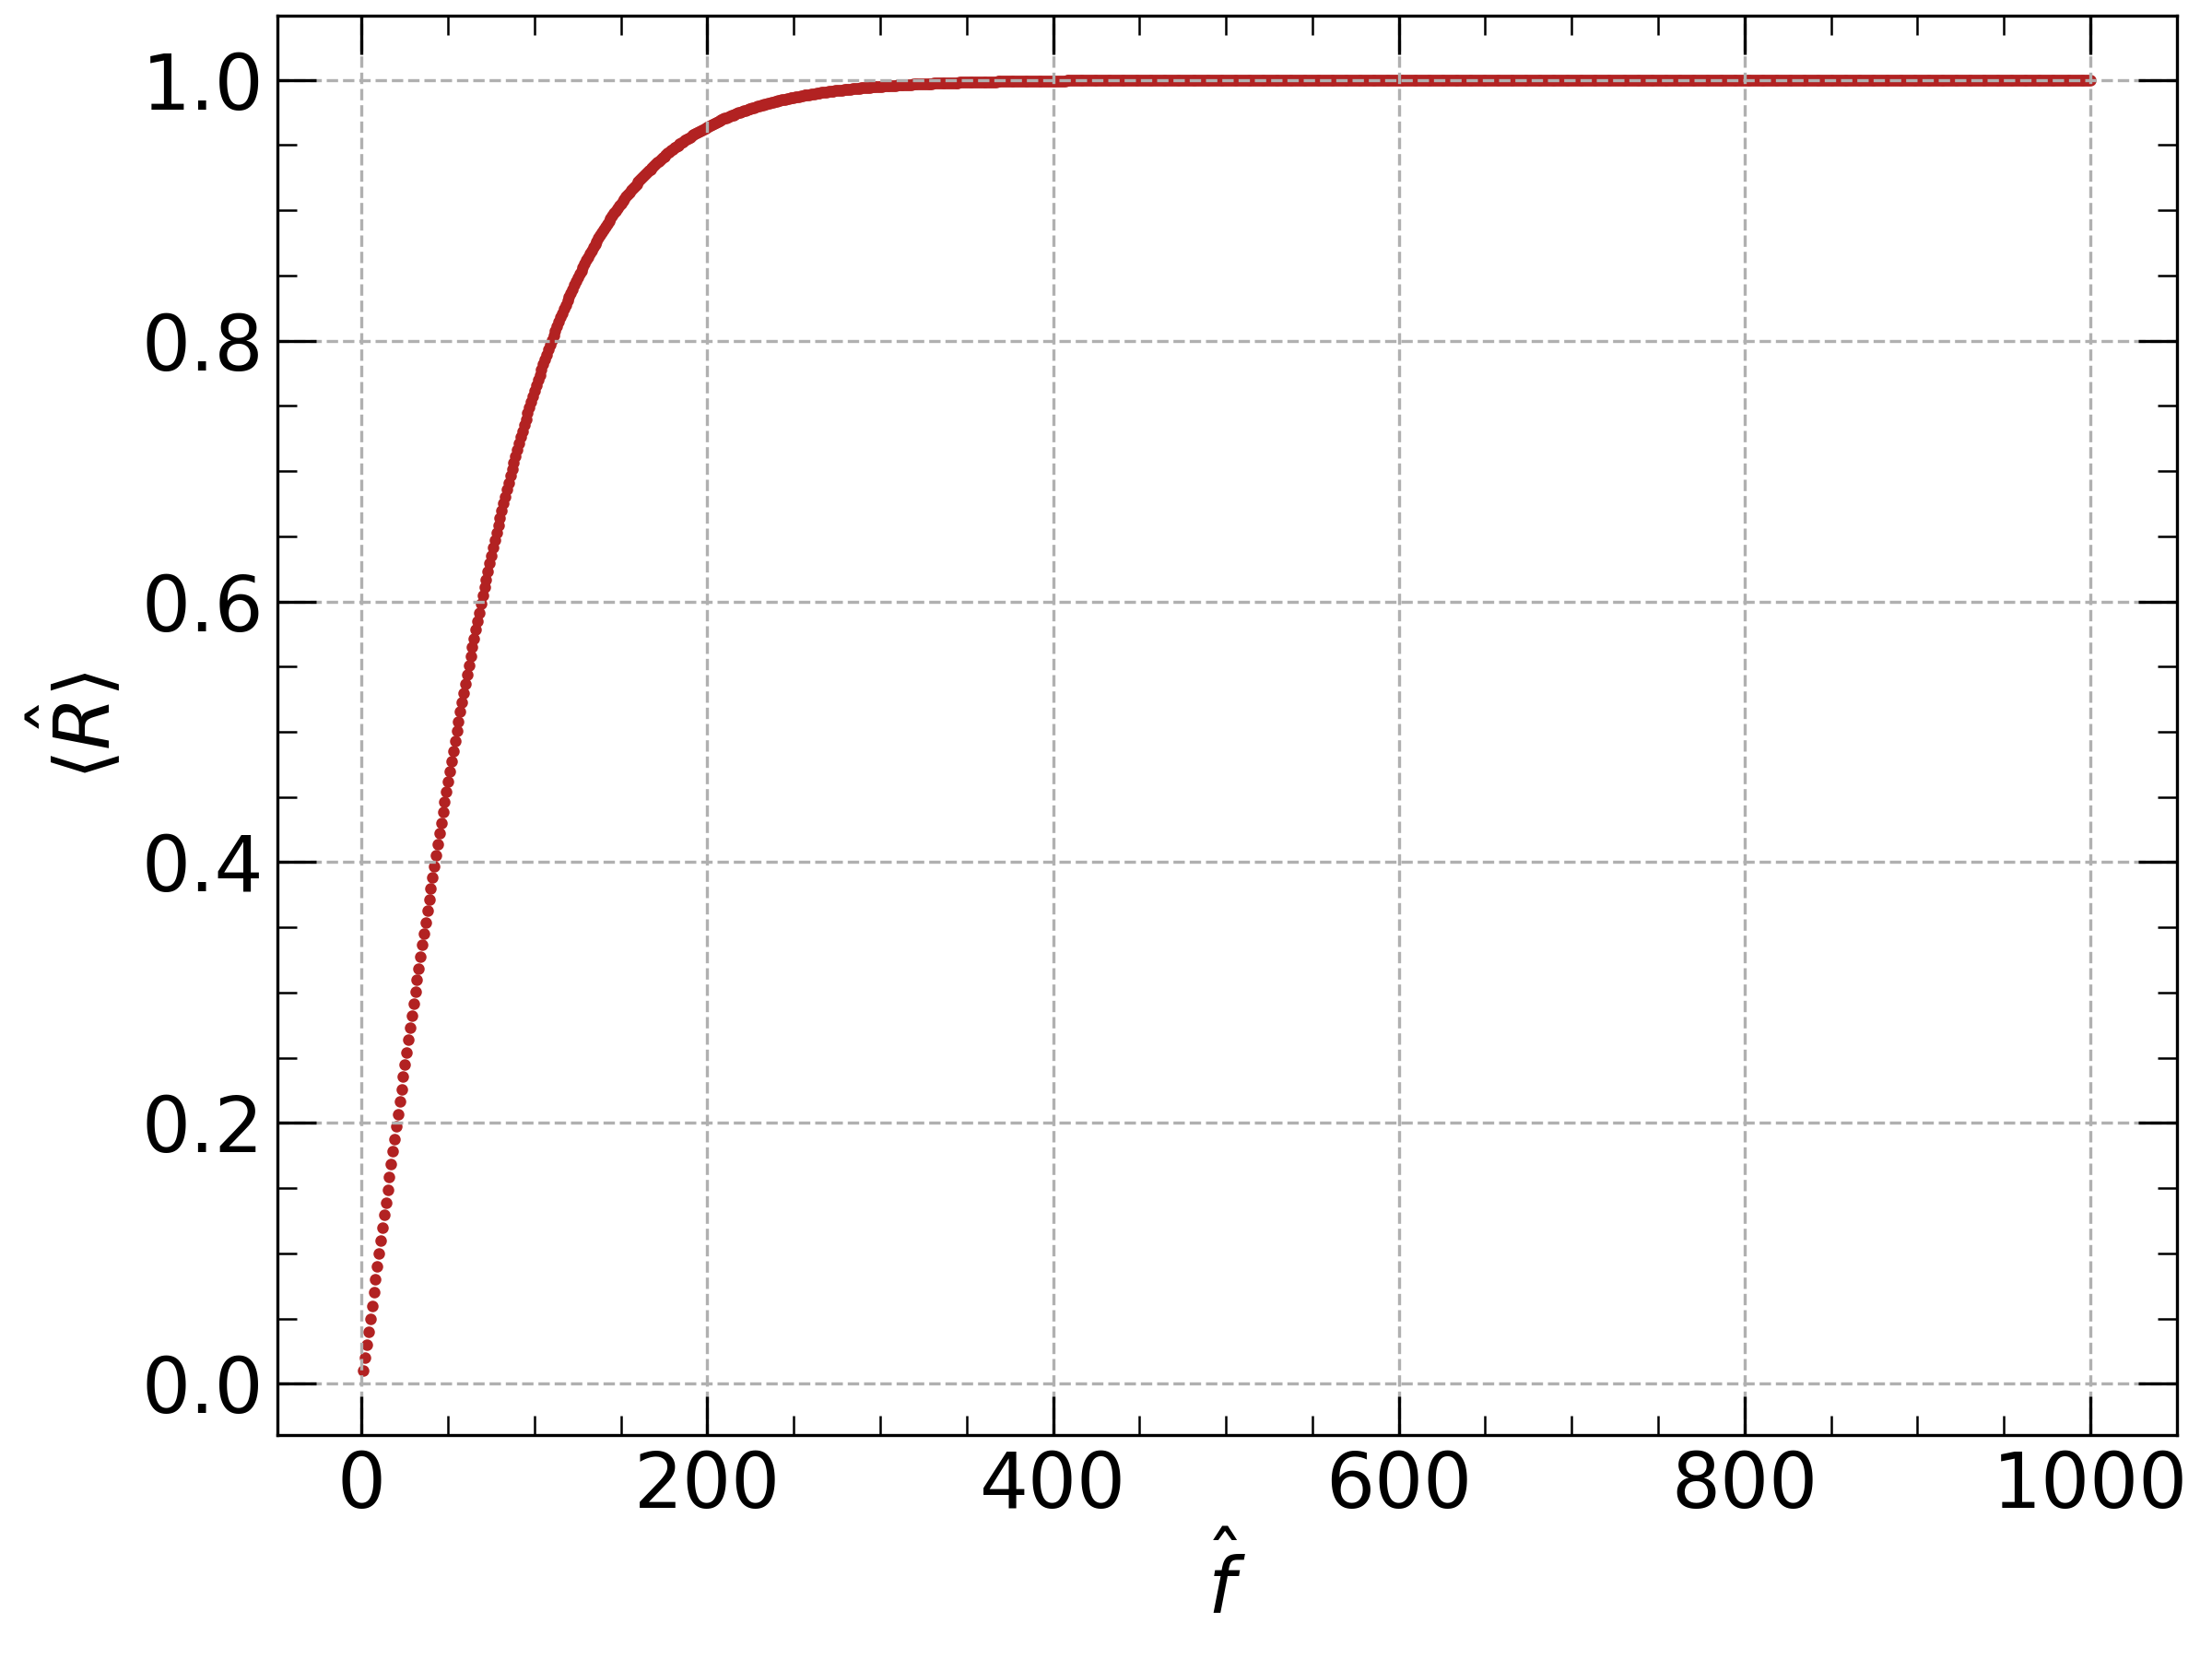
\includegraphics[width=\textwidth]{../../Lliurament_2/document_L2/plots/canvi_f.png}
         \caption{}
         \label{fig:força}
    \end{subfigure}
    \hspace{0.7cm}
    \begin{subfigure}[b]{0.45\textwidth}
        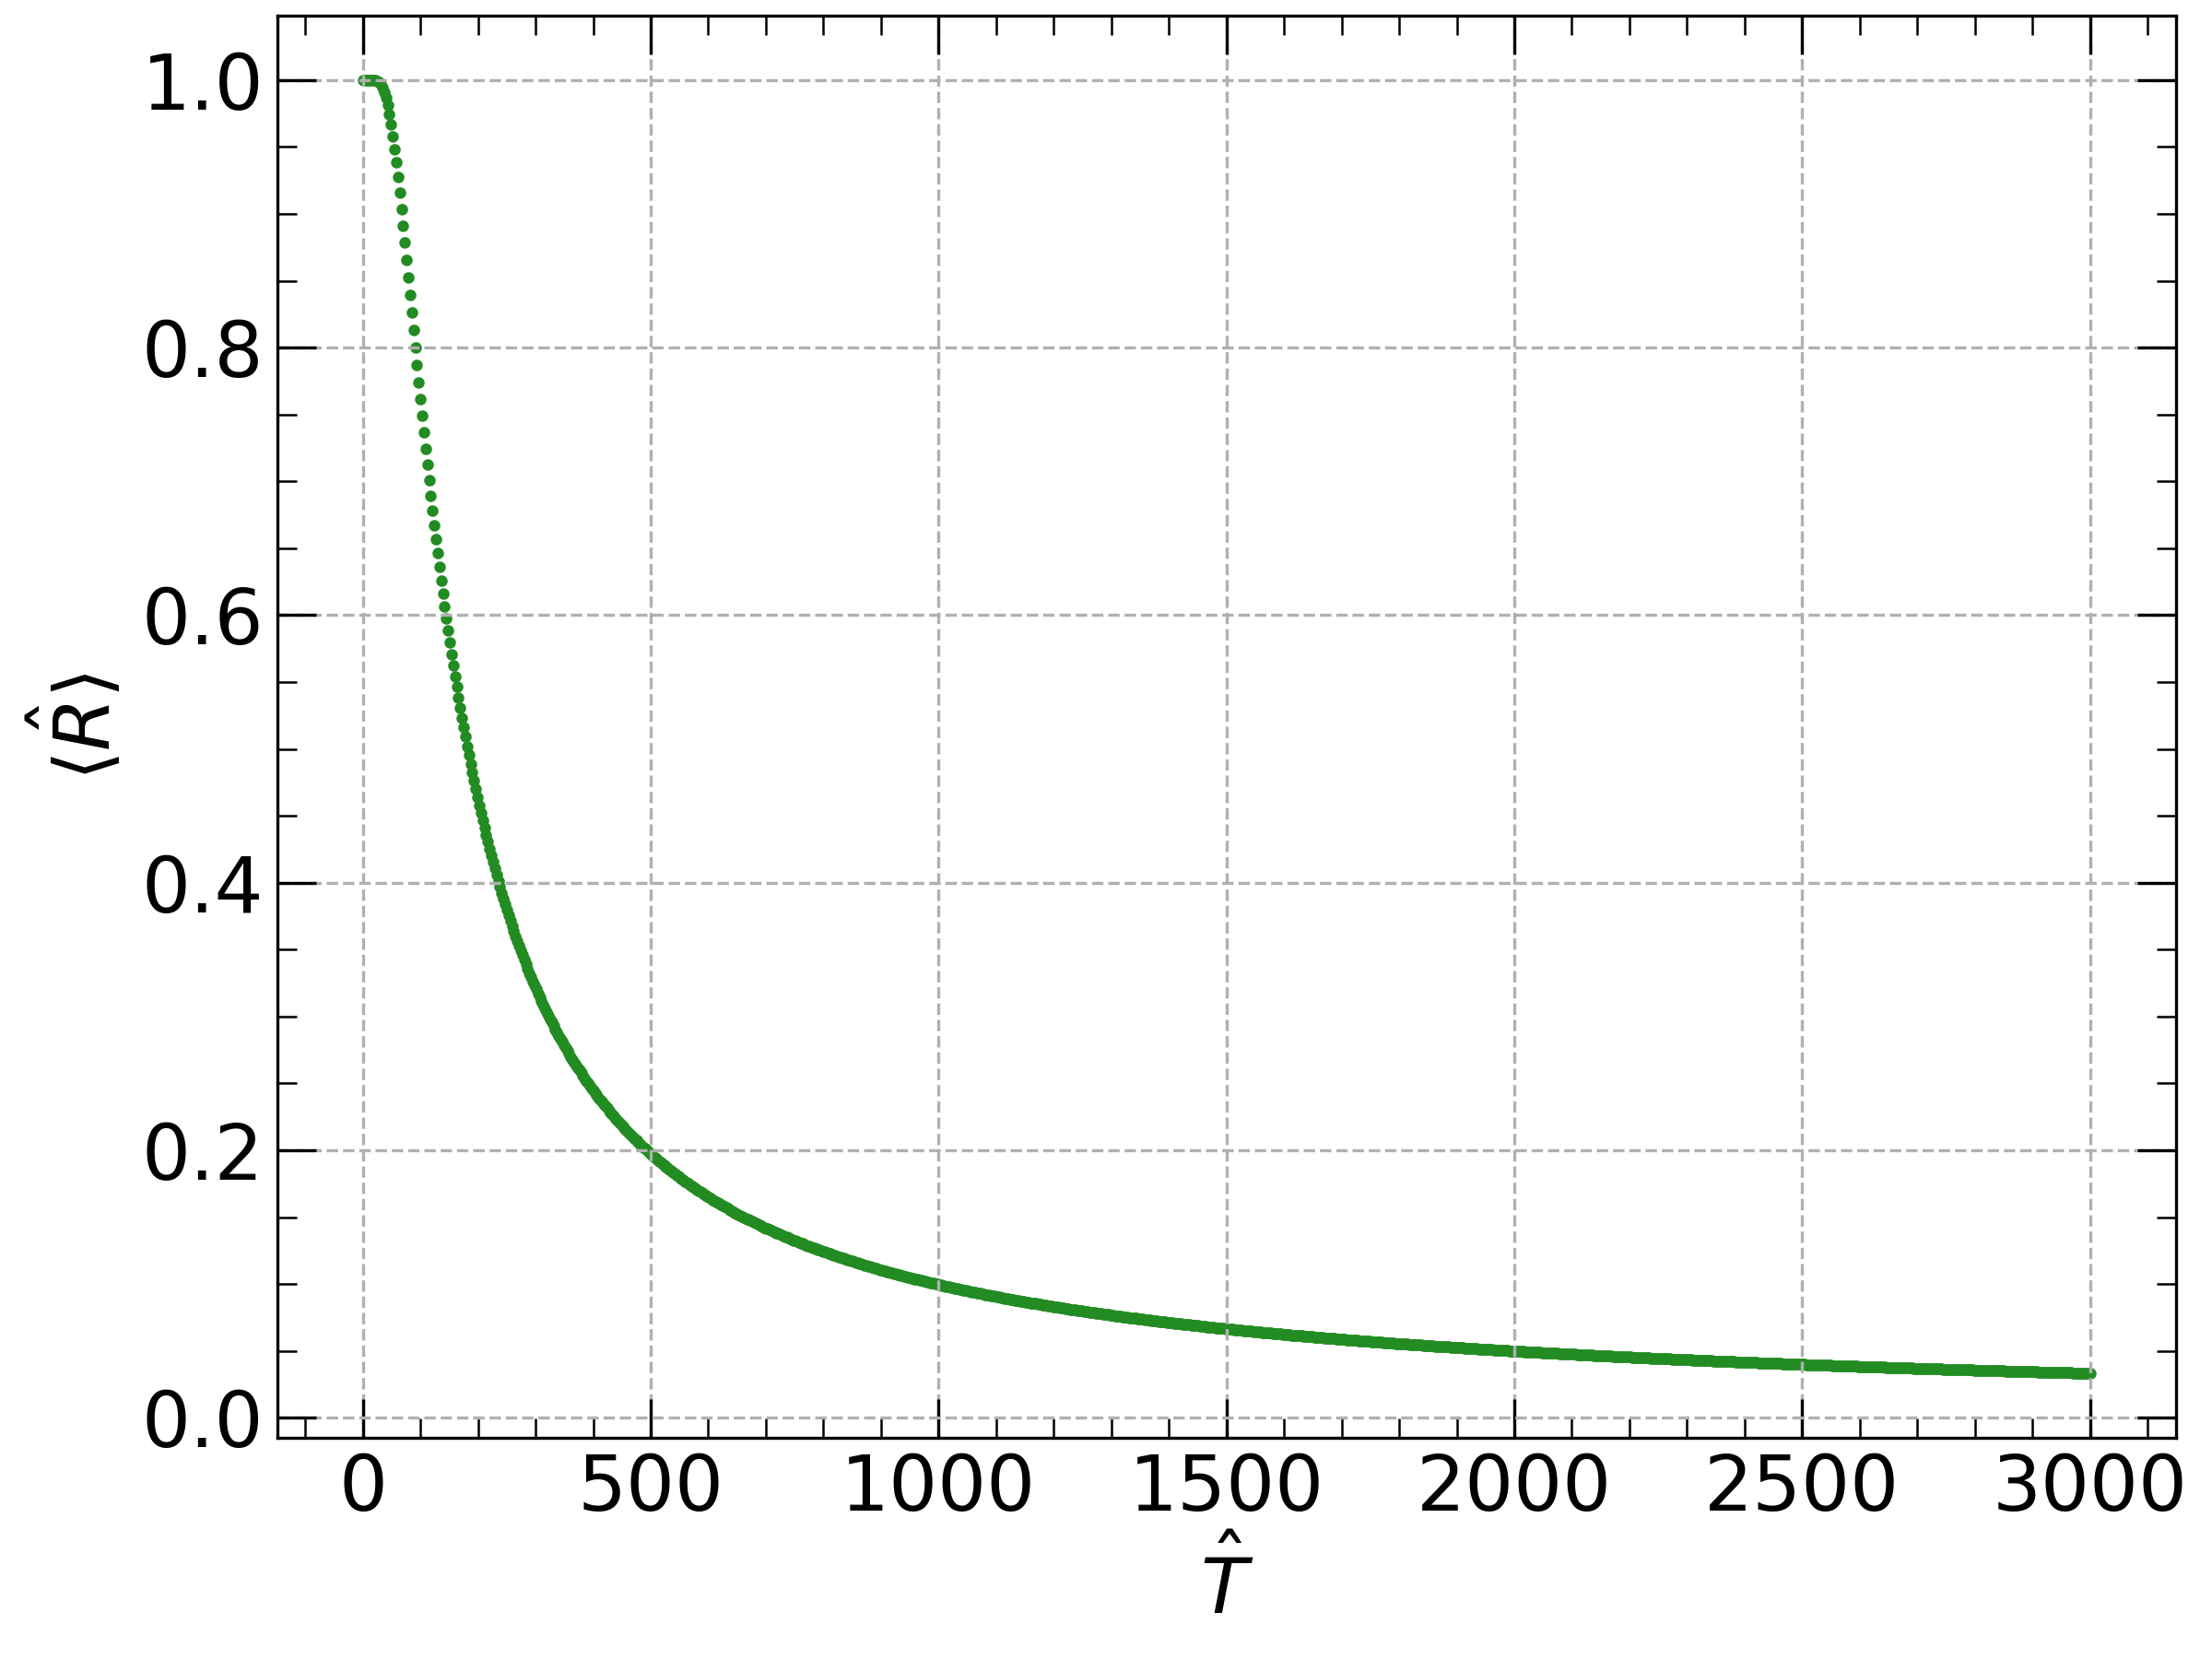
\includegraphics[width=\textwidth]{../../Lliurament_2/document_L2/plots/canvi_T.png}
        \caption{}
        \label{fig:temperatura}
   \end{subfigure}
   \caption{\footnotesize a) Evolució de $\langle \hat{R} \rangle$ respecte $\hat{f}$, escollint $k_{\text{B}}T_{\text{fix}} = 100\,\text{J}$ b) Evolució de $\langle \hat{R} \rangle$ respecte $\hat{T}$, escollint $lf_{\text{fix}} = 100 \, \text{J}$.}
   \label{fig:2D}
\end{figure}
S'observa a la Subfigura \ref{fig:força} com la longitud augmenta amb la força fins a arribar a la longitud màxima (en aquest cas al se adimensional arriba a 1). Per altra banda a la Subfigura \ref{fig:tempertura} es veu com la longitud disminueix amb l'augment de temperatura. Ens podem fixar també en aquesta subfigura com a l'inici, a baixa temperatura, existeix un petit interval on $\langle \hat{R} \rangle$ decau molt més lentament que a la resta de temperatures. Això és deu a què en aquest petit interval la temperatura ha de contrarrestar l'efecte de la força externa aplicada.\\\\
Per a poder observar millor aquestes dependències, podem graficar en tres dimensions com varia $\langle \hat{R} \rangle$ segons les coordenades ($\hat{f}, \hat{T}$). Redefinim les variables $\hat{f}$ i $\hat{T}$ com a variables amb dimensions d'energia, és a dir, $\hat{f} = lf$ i $\hat{T} = k_{\text{B}}T$.\\\\
Per tal de representar-ho de forma que es mostrin els canvis que hem comentat, escollim com els valors de $\hat{f}$ i $\hat{T}$ entre \(200\,\text{J}\) i \(1000\,\text{J}\). S'observa aquesta representació a la Figura \ref{fig:3D}.
\newpage
\begin{figure}[h]
    \centering
    \begin{subfigure}[b]{0.48\textwidth}
         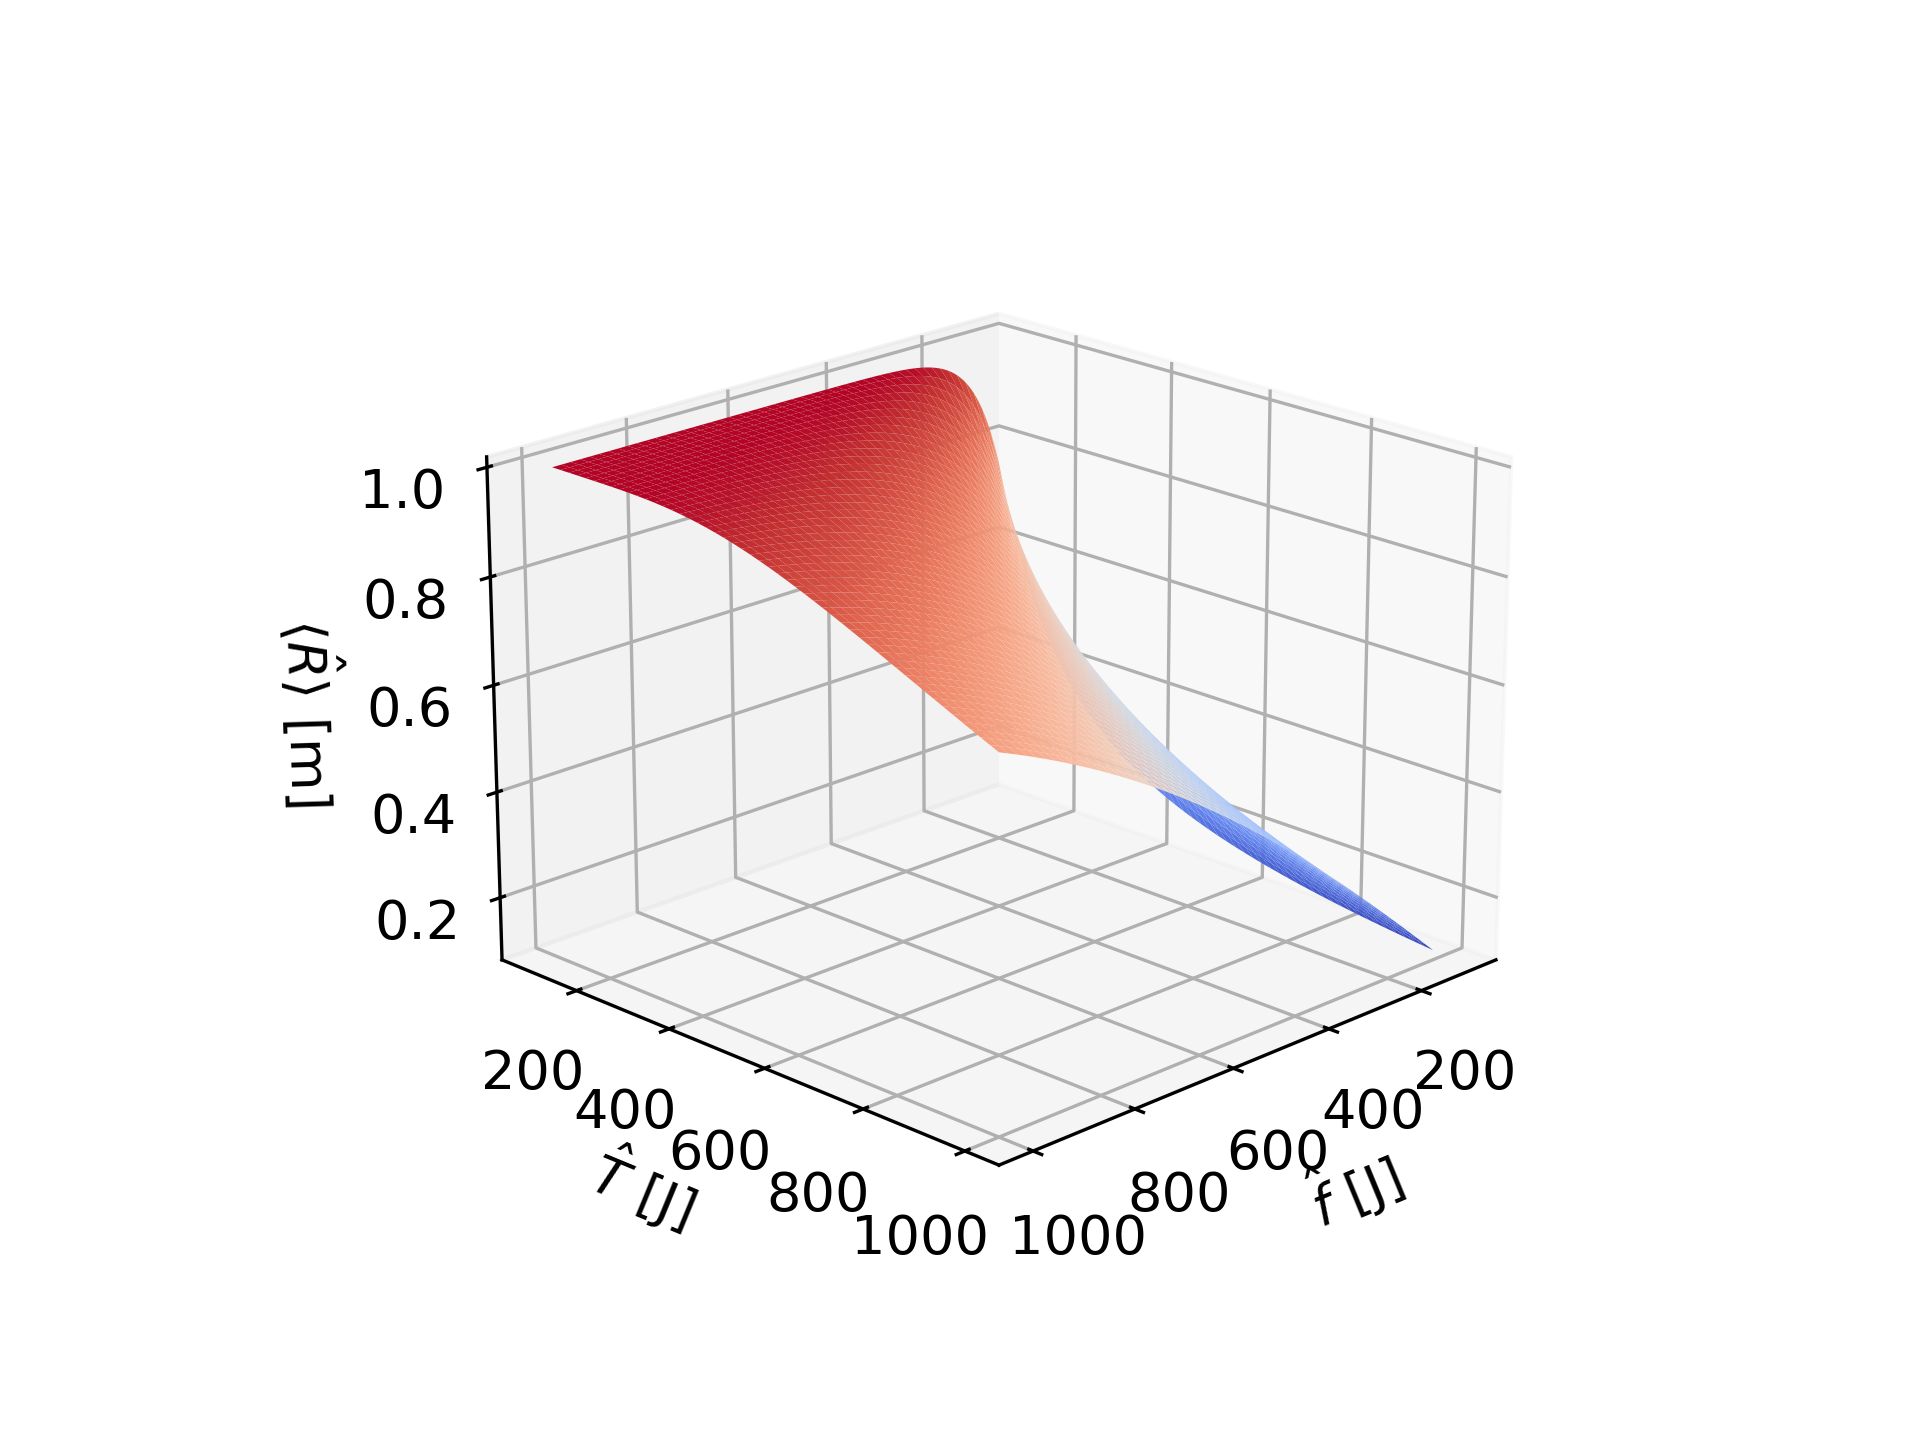
\includegraphics[width=\textwidth]{../../Lliurament_2/document_L2/plots/canvi_3D_45.png}
         \caption*{$\phi= \pi/4$}
         \label{fig:45}
    \end{subfigure}
    \hspace{0.3cm}
    \begin{subfigure}[b]{0.48\textwidth}
        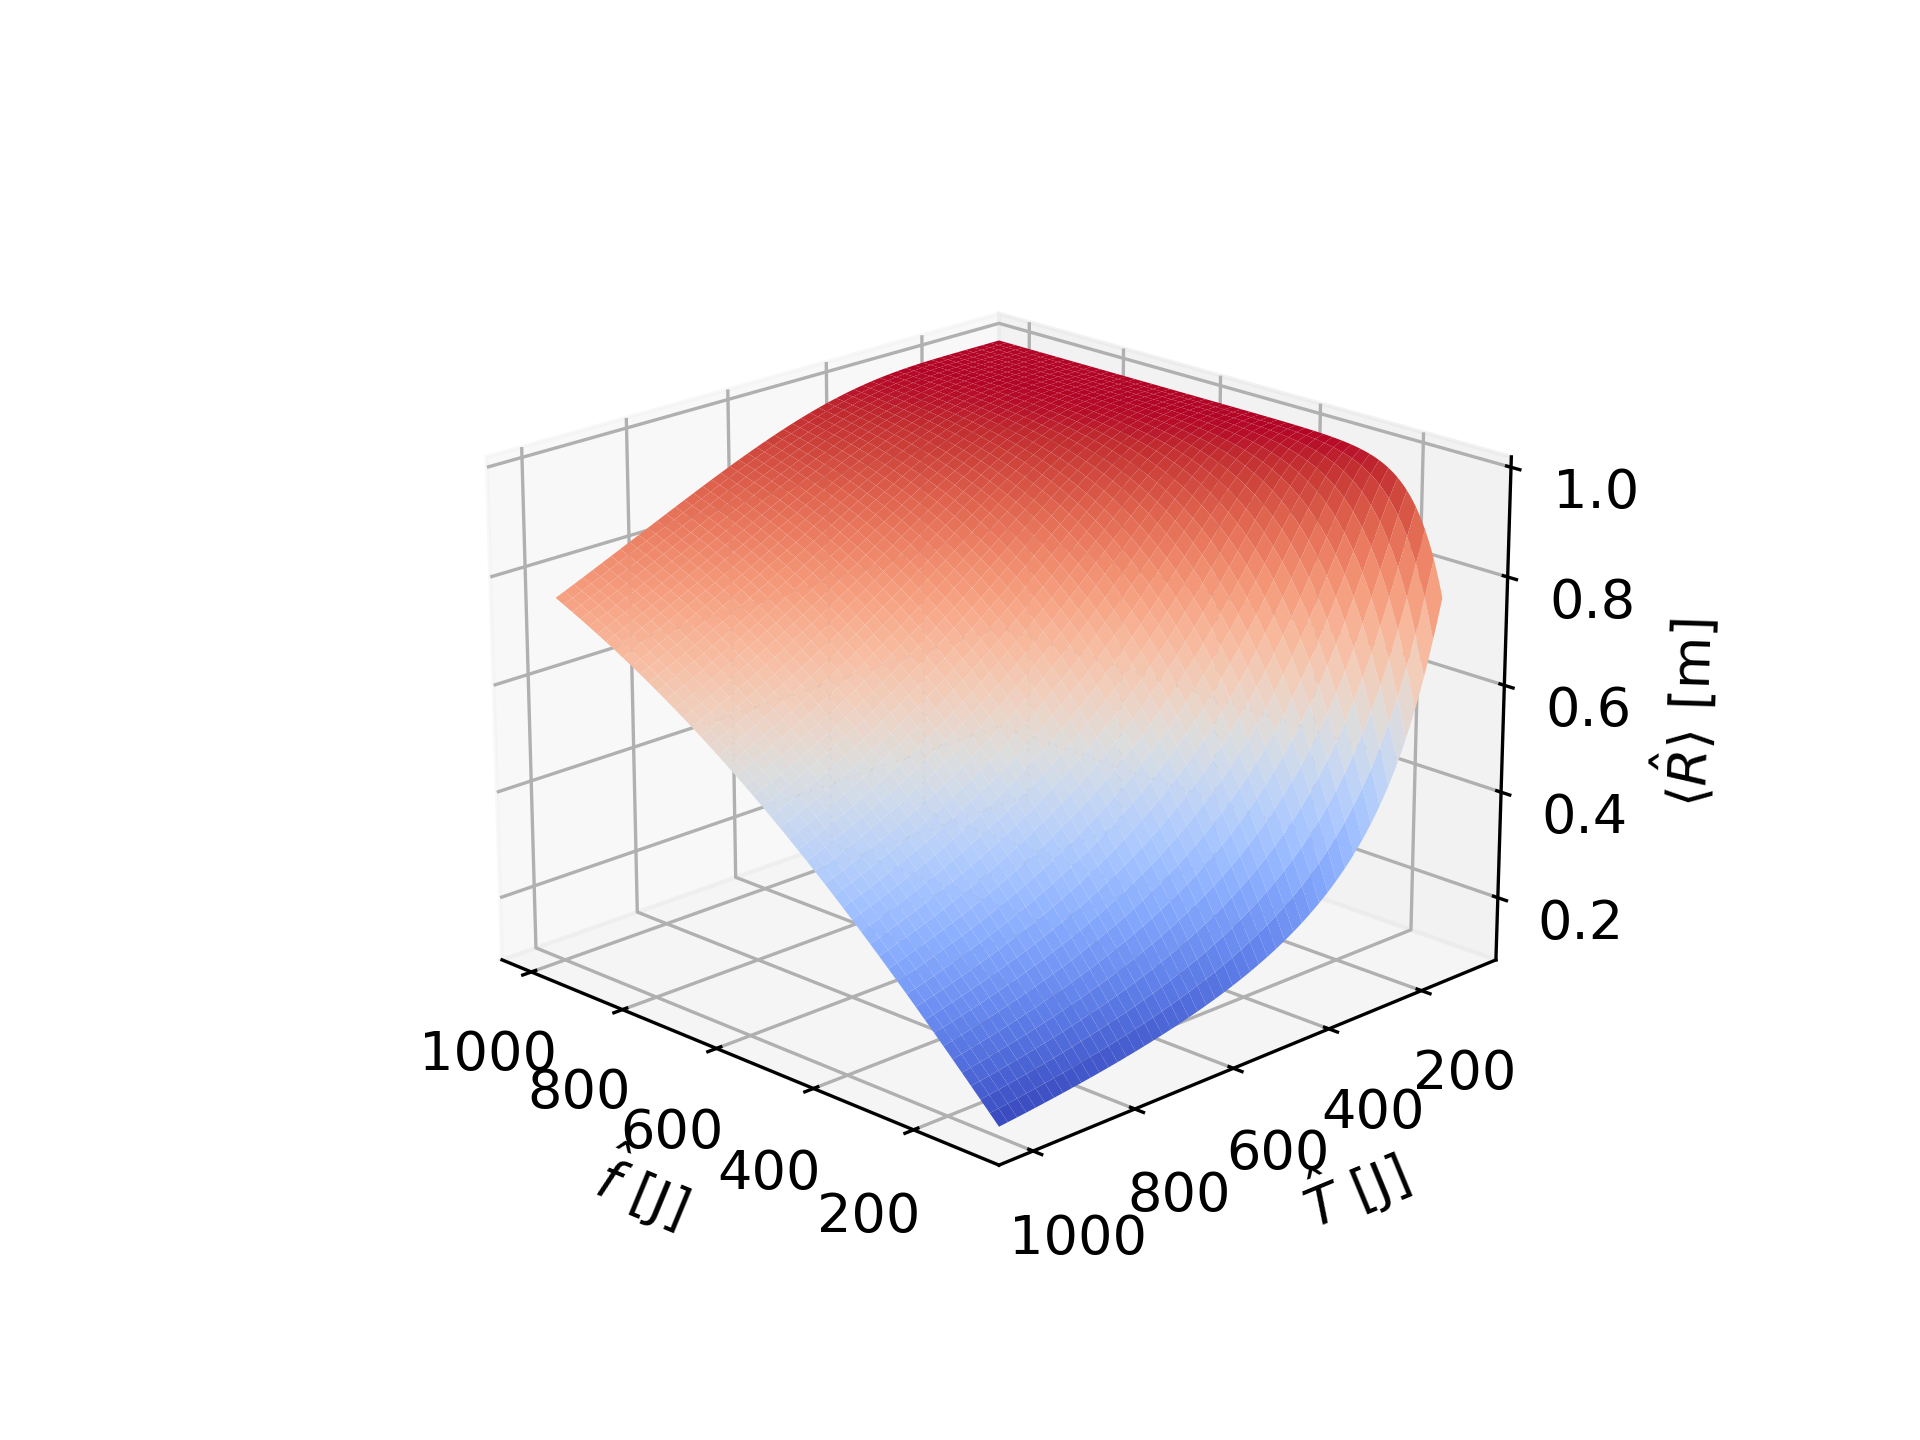
\includegraphics[width=\textwidth]{../../Lliurament_2/document_L2/plots/canvi_3D_135.png}
        \caption*{$\phi= 3\pi/4$}
        \label{fig:135}
    \end{subfigure}
    \begin{subfigure}[b]{0.48\textwidth}
         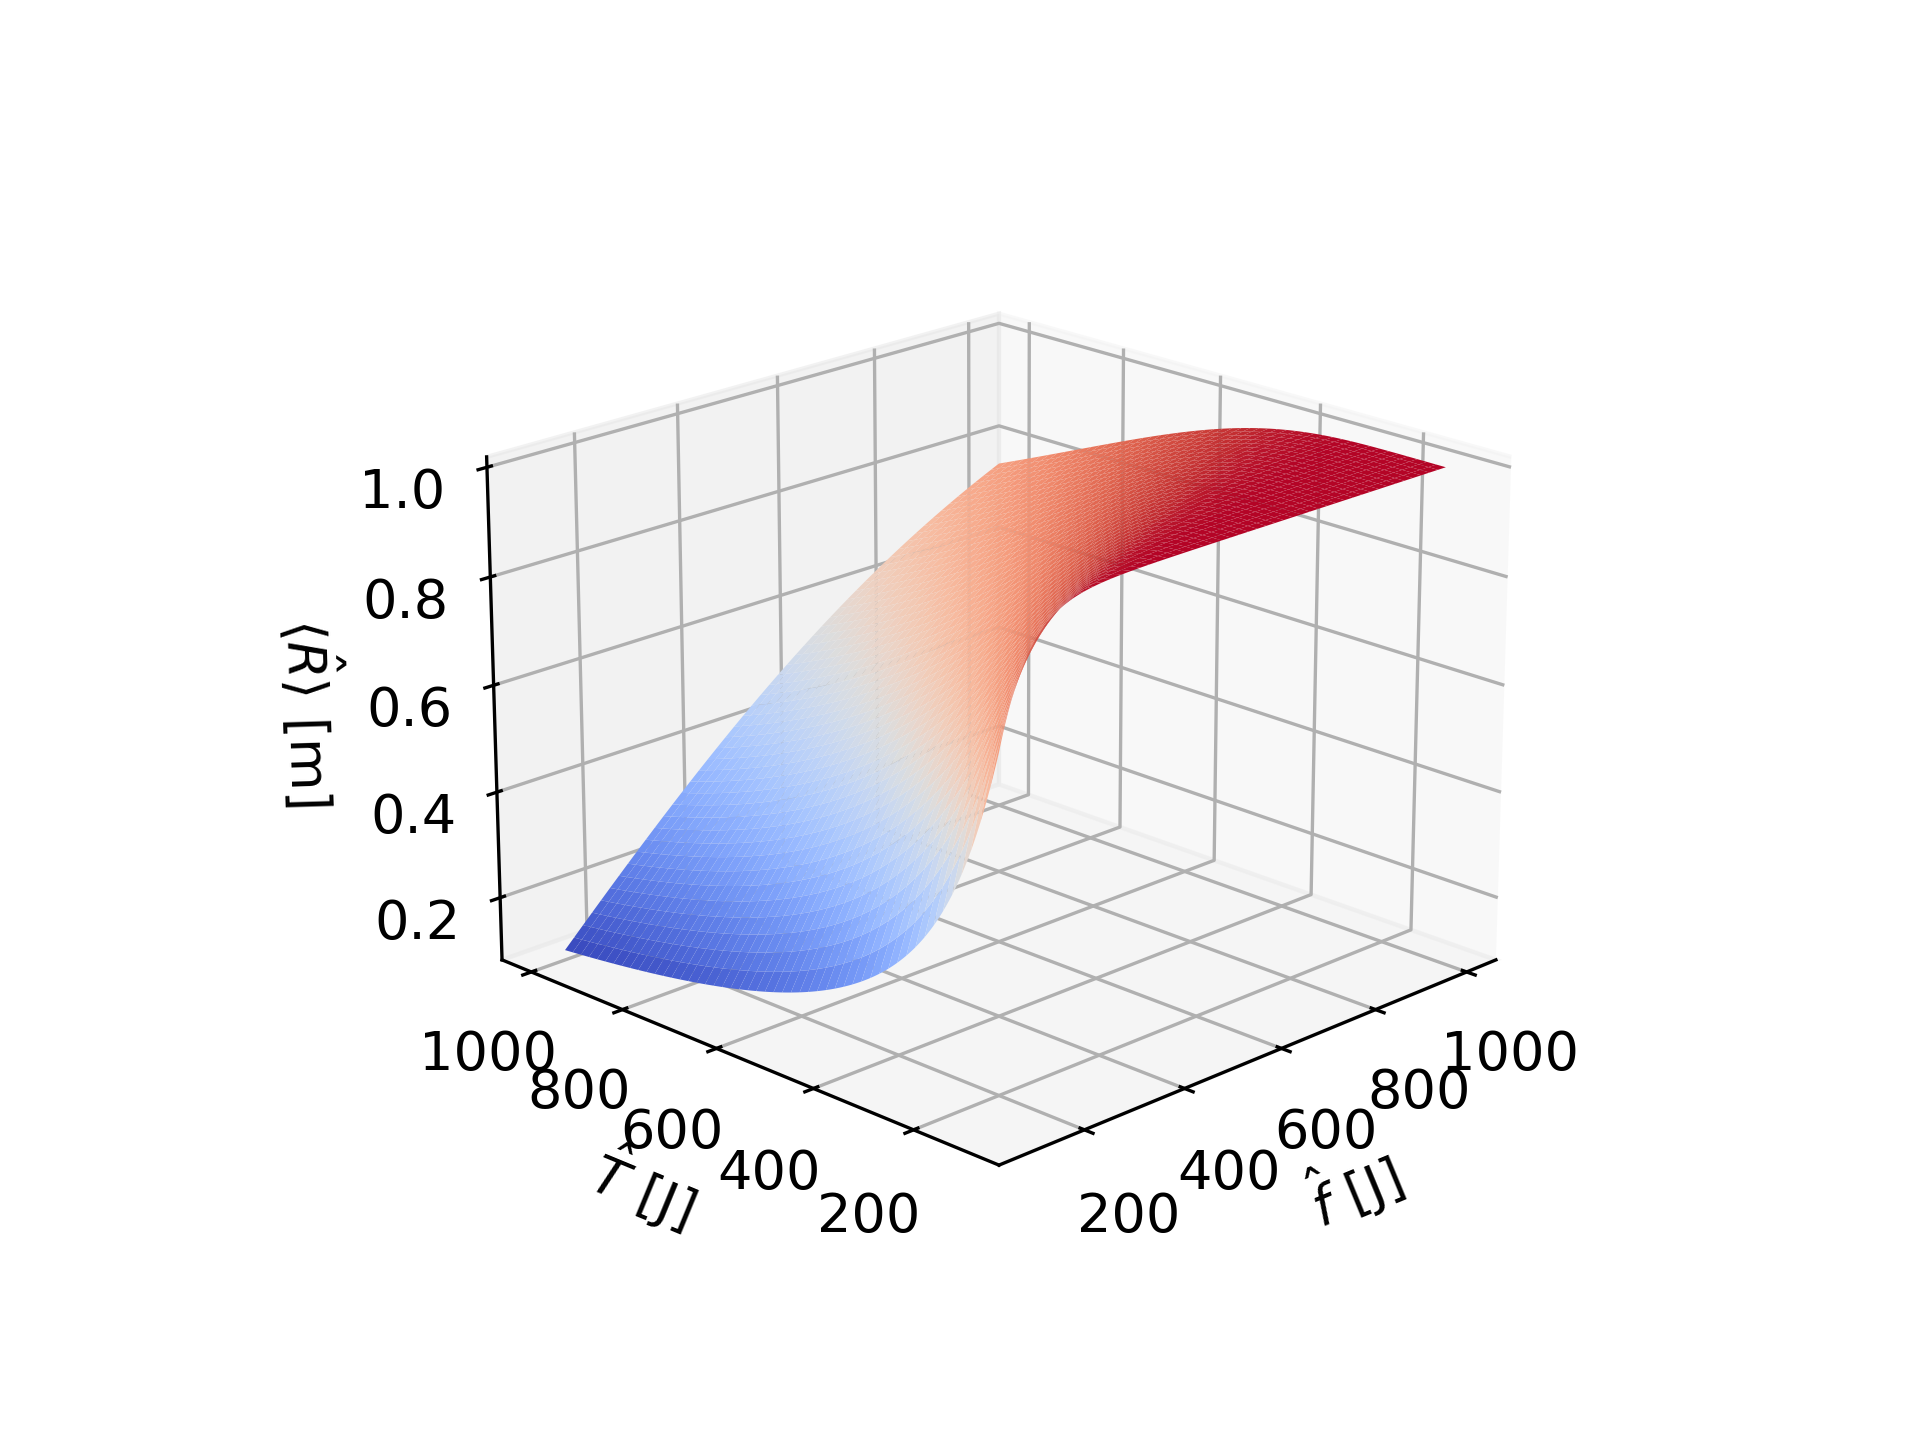
\includegraphics[width=\textwidth]{../../Lliurament_2/document_L2/plots/canvi_3D_225.png}
         \caption*{$\phi= 5\pi/4$}
         \label{fig:225}
    \end{subfigure}
    \hspace{0.3cm}
    \begin{subfigure}[b]{0.48\textwidth}
        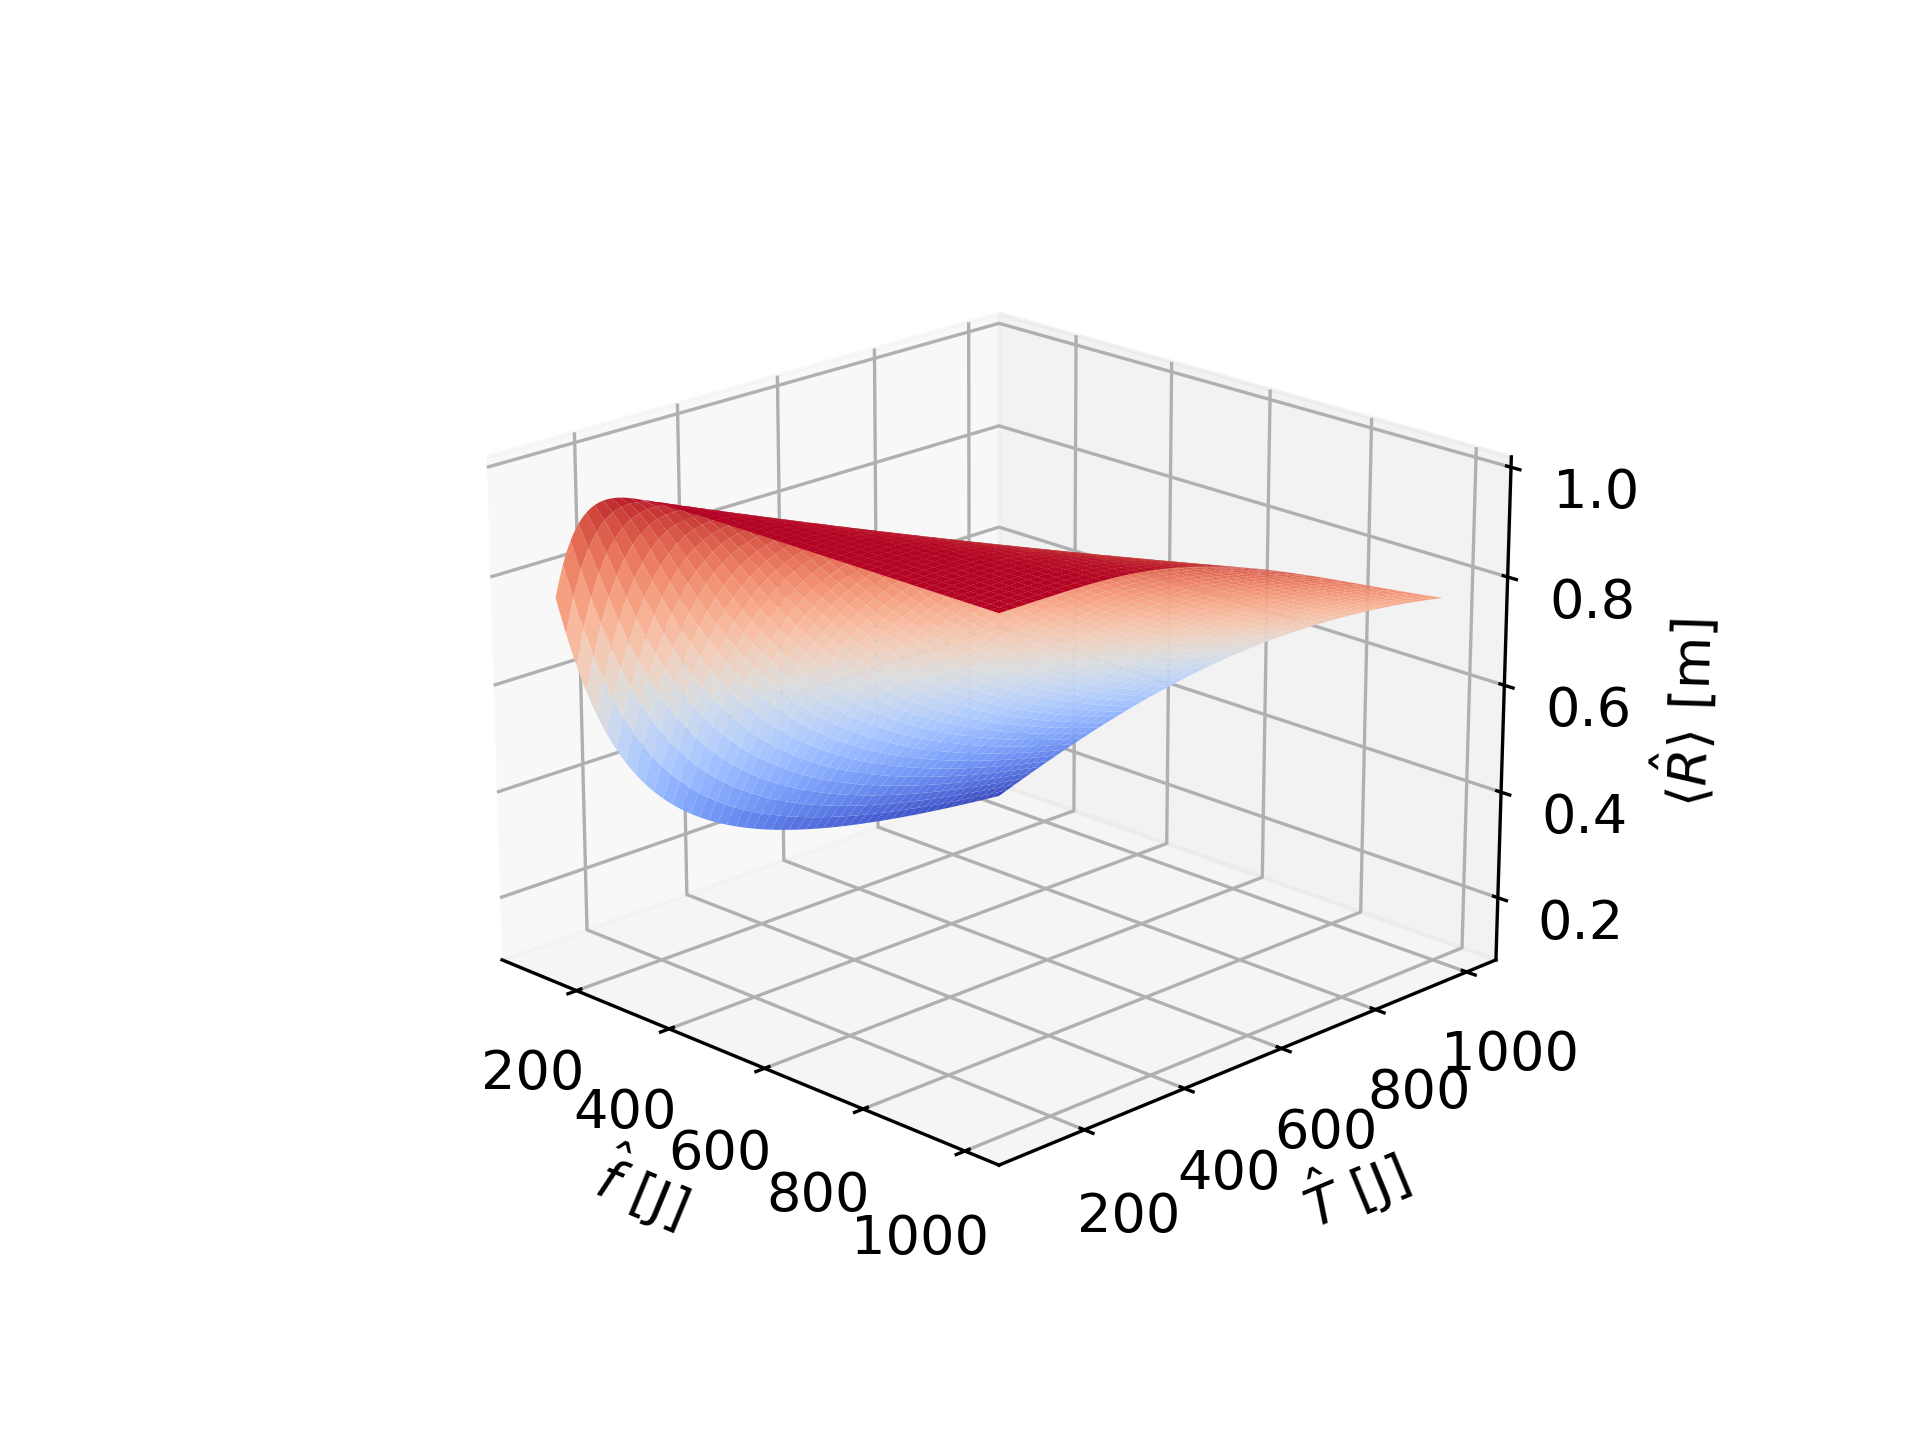
\includegraphics[width=\textwidth]{../../Lliurament_2/document_L2/plots/canvi_3D_315.png}
        \caption*{$\phi= 7\pi/4$}
        \label{fig:215}
    \end{subfigure}
    \caption{\footnotesize Repressentació en 3D de la variació de $\langle \hat{R} \rangle$ segons $\hat{f}$ i $\hat{T}$ en un rang de \(200\,\text{J}\) a \(1000\,\text{J}\). L'angle $\phi$ és l'angle azimutal, es representa en diferents valors per a canviar de perspectiva.}
    \label{fig:3D}
\end{figure}
\noindent Addicionalment es deixa un gif animat on s'observa al complet el gràfic representat a un repositori de GitHub. L'enllaç per a accedir-hi és \url{https://github.com/Efesic/TiME}, i es pot trobar dins del següent directori: \texttt{Lliurament\_2/animacio\_L2.gif}\\\\
S'observa com, per exemple, el gràfic $\langle \hat{R} \rangle$ vs. $\hat{f}$ varia segons augmenta la temperatura. A un valor de \(\hat{T} = 200 \, \text{J}\) es pot observar la Figura \ref{fig:3D} a la perspectiva de $\phi= 5\pi/4$ com el pla $\langle \hat{R} \rangle$ s'assembla al que es mostra a la Subfigura \ref{fig:força}, l'elongació arriba pràcticament a la longitud màxima. En canvi per a \(\hat{T} = 1000 \, \text{J}\) s'observa un canvi en aquest comportament, ara l'elongació a la qual es pot arribar és menor a la màxima elongació. En realitat augmentant més la força si que s'arriba a aquesta longitud màxima, però el gràfic queda tallat abans que això passi.\\\\
Tot i que s'observa pitjor, es pot veure que aquest canvi també passa si comparem la gràfica 3D amb la Subfigura \ref{fig:temperatura}. S'observa a la Figura \ref{fig:3D} a la perspectiva de $\phi= 3\pi/4$ com a \(\hat{f} = 200 \, \text{J}\) es mostra una corba similar a la que es mostra a la Subfigura \ref{fig:temperatura}. Per a un valor de \(\hat{f} = 1000 \, \text{J}\), es veu a la perspectiva de $\phi= 7\pi/4$ com la temperatura encara encongeix la molècula, però ho fa de forma més lenta.\\\\
Finalment, comprovem en quines condicions és vàlida la llei de Hooke per a la nostra molècula. Sabem de l'exercici anterior (Lliurament 1) que aquesta llei s'expressa com
\begin{equation*}
    f = -kR
\end{equation*}
on $k$ és la constant d'elasticitat. Notem com aquesta llei és lineal respecte a $R$. Per tant, aquesta llei es compleix només per a forçes relativament petites, és a dir, quedant-nos a primer ordre de la funció $\tanh{(x)} \simeq x$:
\begin{equation*}
    \hat{f} \simeq \hat{T} \langle \hat{R} \rangle
\end{equation*}
Observem com $k$ correspon al pendent de la corba $\langle \hat{R} \rangle$ vs. $\hat{f}$ per a forces petites, on es pot aproximar a una recta. Concloem que la llei de Hooke és vàlida per a forces relativament petites i que depèn de la temperatura.
\end{document}